\section{Introduction}

CMS experiment computing \cite{cmscomptdr} infrastructure spans over more than a hundred 
of geographically distributed sites that provide both computational and data storage 
resources. Storage capacity at the sites varies from hundreds terabytes to several petabytes. 
During the first LHC run, CMS data saturated hundred petabytes of storage. 
Data taking rate and total data volume will be substantially increased during the Run 2.

\begin{figure}[h]
\center
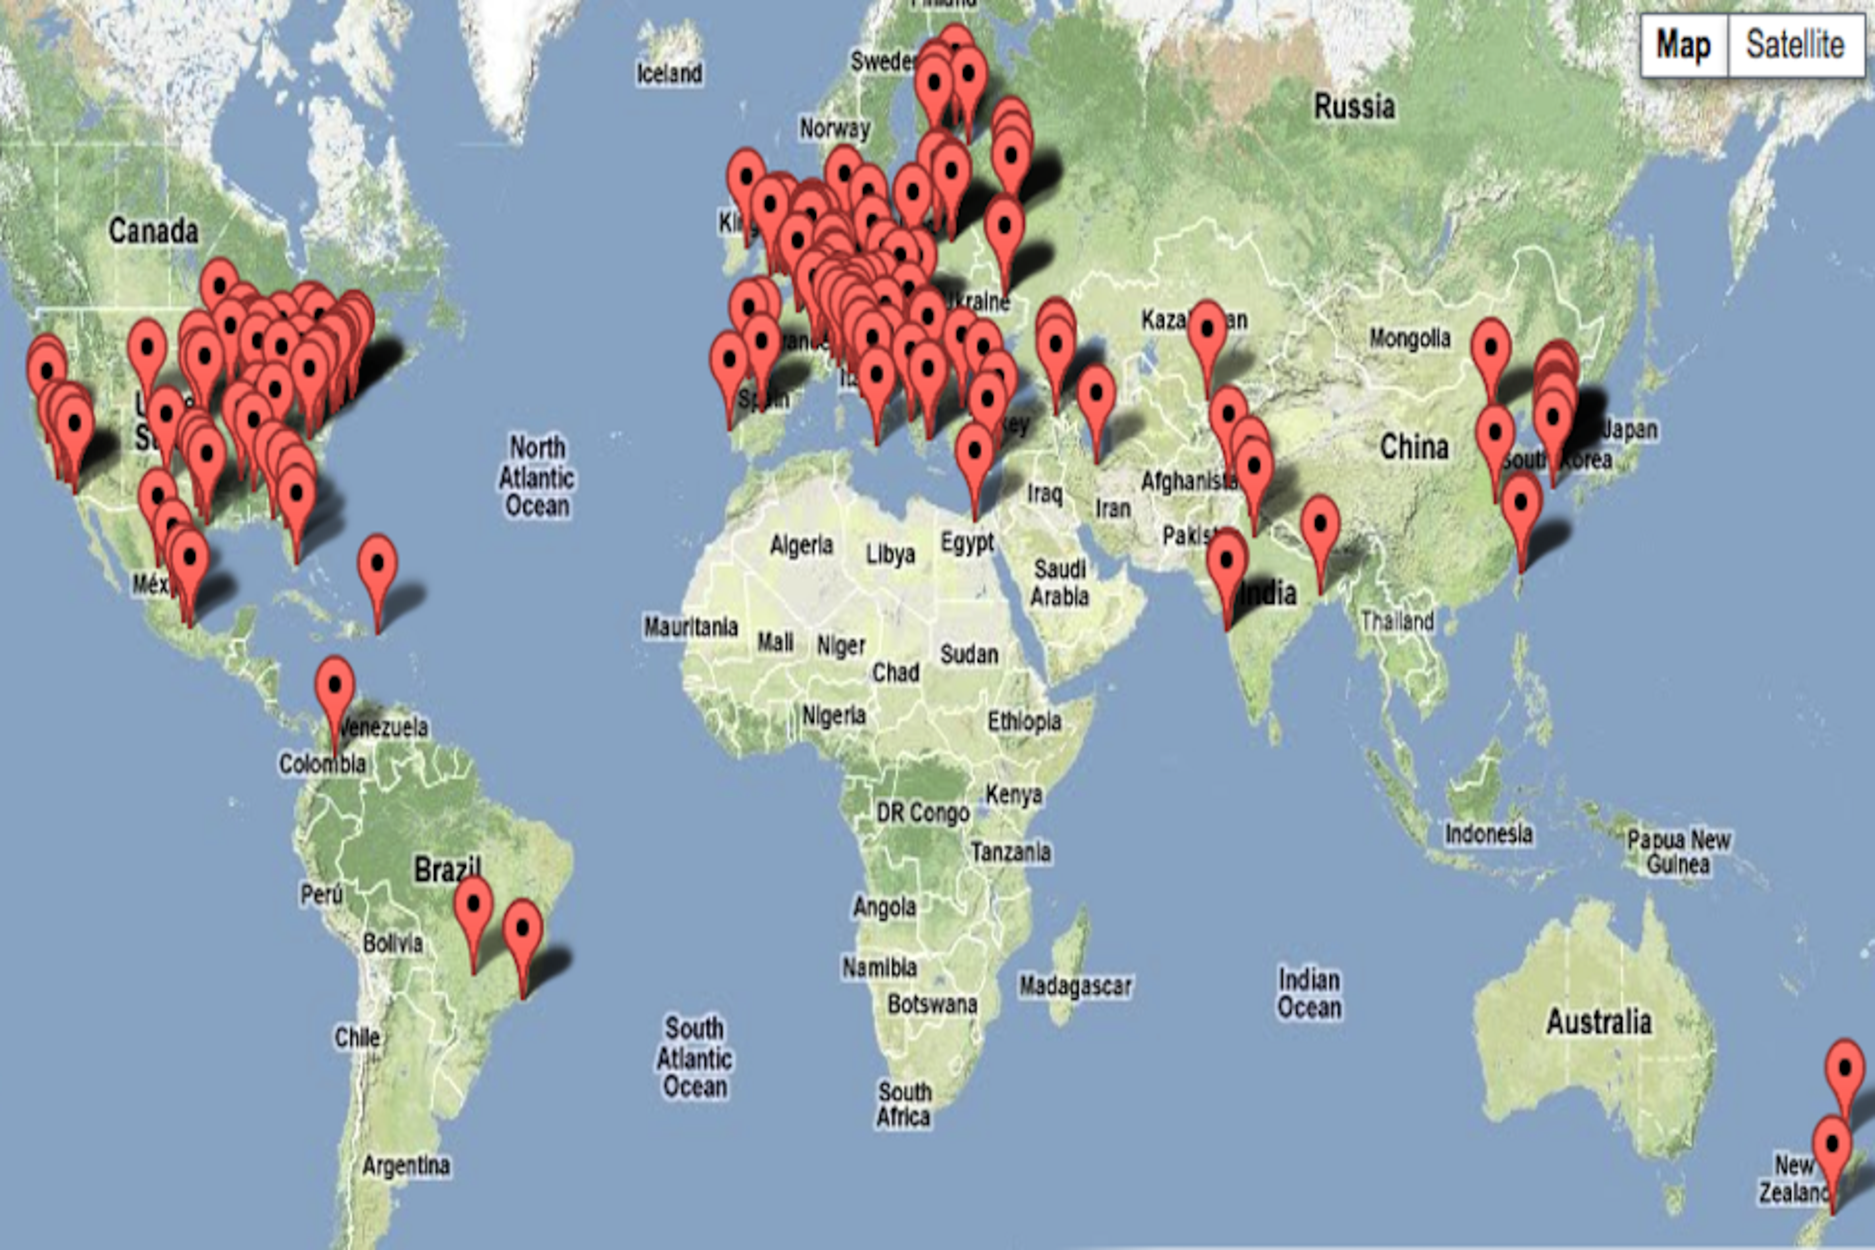
\includegraphics[width=0.95\linewidth]
{pictures/cms-sites-map.pdf}
\caption{World map showing locations of CMS collaborating universities and institutes}
\label{fig:sites_map}
\end{figure}

Storage accounting and space monitoring becomes increasingly important for data 
management tasks, such as efficient space utilization, fair share between users and 
groups, and resource planning.

Data stored at the sites are coming from a variety of sources and include i) centrally managed 
data sets such as real detector data and simulated data samples at various stages of reprocessing, 
software release validation samples; ii) files created by individual 
users or members of physics analysis groups stored at the associated institute sites; 
iii) temporary unmerged files generated as part of the data processing workflows; 
iiii) load test and backfill data used for availability and scalability testing \cite{scalability}.

CMS space monitoring system, SpaceMon \cite{spacemon}, provides monitoring for storage space 
occupied by various directories in the CMS data directory tree. 

Information is retrieved directly from the local site storage systems in the form of 
storage dumps produced by various methods or tools depending on the storage technology and
local sites infrastructure, following a commonly agreed format \cite{storagedumps}.

The CMS data management system \cite{cmsdatamanagement} keeps track the centrally managed 
file replicas in the central data transfer management database. The SpaceMon information 
collected at the sites allows to account additional storage space used by the users 
and groups, and various other volatile data areas, not tracked in the central catalogs.

The information is aggregated locally at the sites, then uploaded into a central database at CERN.

In section 2 we discuss site information providers process and tools. Sections 3 and 4 describe 
SpaceMon client software and the components of the central infrastructure.
In concluding sections we present project's current status and our experience of SpaceMon deployment 
at CMS sites.
